% Created by tikzDevice version 0.12.6 on 2026-07-06 23:55:43
% !TEX encoding = UTF-8 Unicode
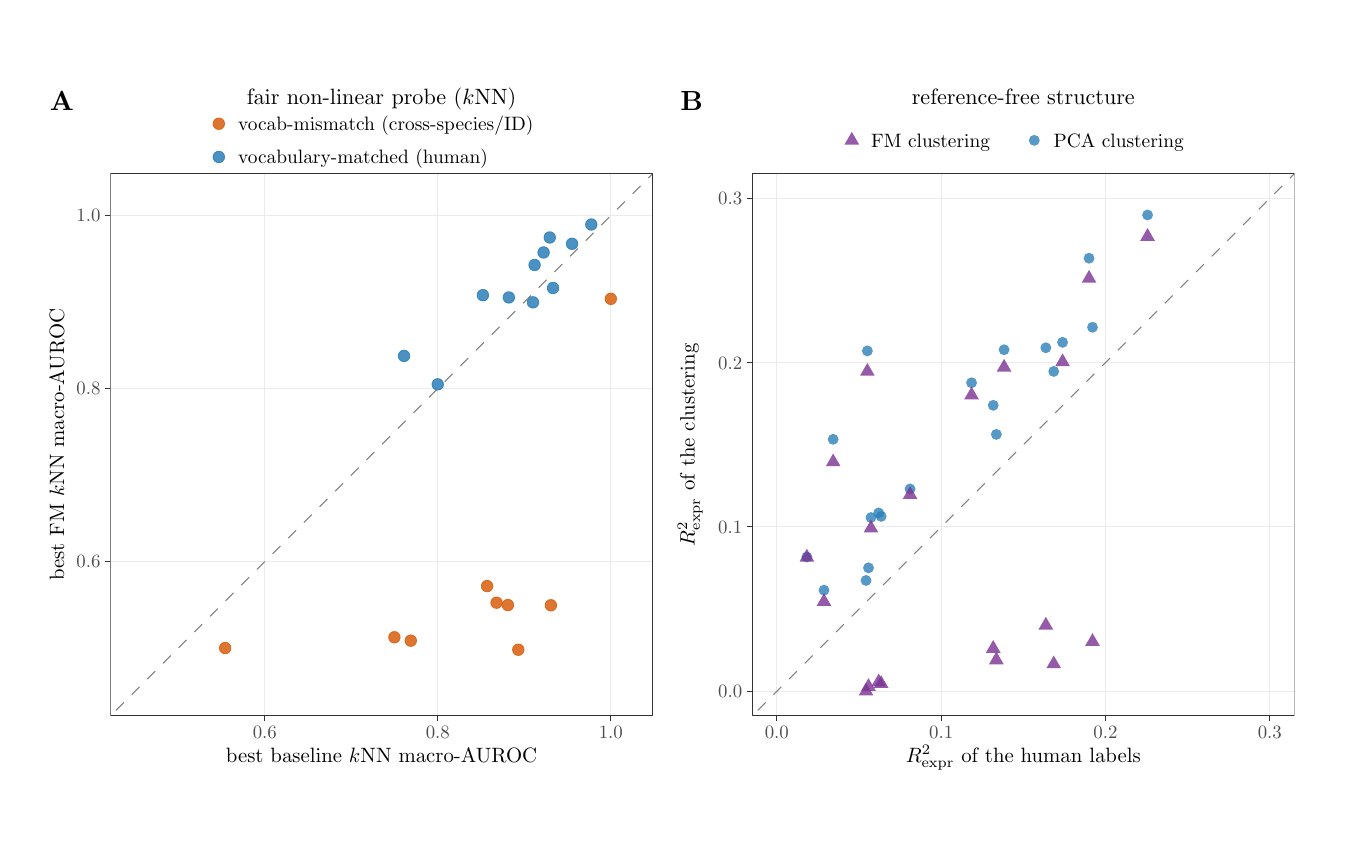
\begin{tikzpicture}[x=1pt,y=1pt]
\definecolor{fillColor}{RGB}{255,255,255}
\path[use as bounding box,fill=fillColor,fill opacity=0.00] (0,0) rectangle (469.75,289.08);
\begin{scope}
\path[clip] (  0.00, 16.16) rectangle (469.75,272.92);
\definecolor{drawColor}{RGB}{255,255,255}
\definecolor{fillColor}{RGB}{255,255,255}

\path[draw=drawColor,line width= 0.4pt,line join=round,line cap=round,fill=fillColor] ( -0.00, 16.16) rectangle (469.76,272.92);
\end{scope}
\begin{scope}
\path[clip] (  4.00, 19.16) rectangle (231.88,269.92);
\definecolor{drawColor}{RGB}{255,255,255}
\definecolor{fillColor}{RGB}{255,255,255}

\path[draw=drawColor,line width= 0.4pt,line join=round,line cap=round,fill=fillColor] (  4.00, 19.16) rectangle (231.88,269.92);
\end{scope}
\begin{scope}
\path[clip] (231.88, 19.16) rectangle (463.75,269.92);
\definecolor{drawColor}{RGB}{255,255,255}
\definecolor{fillColor}{RGB}{255,255,255}

\path[draw=drawColor,line width= 0.4pt,line join=round,line cap=round,fill=fillColor] (231.88, 19.16) rectangle (463.75,269.92);
\end{scope}
\begin{scope}
\path[clip] ( 29.91, 40.39) rectangle (225.88,236.36);
\definecolor{fillColor}{RGB}{255,255,255}

\path[fill=fillColor] ( 29.91, 40.39) rectangle (225.88,236.36);
\definecolor{drawColor}{gray}{0.92}

\path[draw=drawColor,line width= 0.4pt,line join=round] ( 29.91, 96.18) --
	(225.88, 96.18);

\path[draw=drawColor,line width= 0.4pt,line join=round] ( 29.91,158.69) --
	(225.88,158.69);

\path[draw=drawColor,line width= 0.4pt,line join=round] ( 29.91,221.20) --
	(225.88,221.20);

\path[draw=drawColor,line width= 0.4pt,line join=round] ( 85.70, 40.39) --
	( 85.70,236.36);

\path[draw=drawColor,line width= 0.4pt,line join=round] (148.21, 40.39) --
	(148.21,236.36);

\path[draw=drawColor,line width= 0.4pt,line join=round] (210.72, 40.39) --
	(210.72,236.36);
\definecolor{drawColor}{gray}{0.50}

\path[draw=drawColor,line width= 0.4pt,dash pattern=on 4pt off 4pt ,line join=round] (-166.06,-155.58) -- (421.84,432.32);
\definecolor{drawColor}{RGB}{44,127,184}
\definecolor{fillColor}{RGB}{44,127,184}

\path[draw=drawColor,draw opacity=0.85,line width= 0.3pt,line join=round,line cap=round,fill=fillColor,fill opacity=0.85] (186.43,207.85) circle (  2.08);

\path[draw=drawColor,draw opacity=0.85,line width= 0.3pt,line join=round,line cap=round,fill=fillColor,fill opacity=0.85] (135.99,170.47) circle (  2.08);
\definecolor{drawColor}{RGB}{217,95,14}
\definecolor{fillColor}{RGB}{217,95,14}

\path[draw=drawColor,draw opacity=0.85,line width= 0.3pt,line join=round,line cap=round,fill=fillColor,fill opacity=0.85] (173.53, 80.43) circle (  2.08);
\definecolor{drawColor}{RGB}{44,127,184}
\definecolor{fillColor}{RGB}{44,127,184}

\path[draw=drawColor,draw opacity=0.85,line width= 0.3pt,line join=round,line cap=round,fill=fillColor,fill opacity=0.85] (148.18,160.19) circle (  2.08);

\path[draw=drawColor,draw opacity=0.85,line width= 0.3pt,line join=round,line cap=round,fill=fillColor,fill opacity=0.85] (173.87,191.60) circle (  2.08);
\definecolor{drawColor}{RGB}{217,95,14}
\definecolor{fillColor}{RGB}{217,95,14}

\path[draw=drawColor,draw opacity=0.85,line width= 0.3pt,line join=round,line cap=round,fill=fillColor,fill opacity=0.85] (166.02, 87.30) circle (  2.08);
\definecolor{drawColor}{RGB}{44,127,184}
\definecolor{fillColor}{RGB}{44,127,184}

\path[draw=drawColor,draw opacity=0.85,line width= 0.3pt,line join=round,line cap=round,fill=fillColor,fill opacity=0.85] (182.59,189.82) circle (  2.08);
\definecolor{drawColor}{RGB}{217,95,14}
\definecolor{fillColor}{RGB}{217,95,14}

\path[draw=drawColor,draw opacity=0.85,line width= 0.3pt,line join=round,line cap=round,fill=fillColor,fill opacity=0.85] (169.43, 81.30) circle (  2.08);
\definecolor{drawColor}{RGB}{44,127,184}
\definecolor{fillColor}{RGB}{44,127,184}

\path[draw=drawColor,draw opacity=0.85,line width= 0.3pt,line join=round,line cap=round,fill=fillColor,fill opacity=0.85] (189.84,195.01) circle (  2.08);

\path[draw=drawColor,draw opacity=0.85,line width= 0.3pt,line join=round,line cap=round,fill=fillColor,fill opacity=0.85] (164.49,192.41) circle (  2.08);

\path[draw=drawColor,draw opacity=0.85,line width= 0.3pt,line join=round,line cap=round,fill=fillColor,fill opacity=0.85] (196.72,210.98) circle (  2.08);

\path[draw=drawColor,draw opacity=0.85,line width= 0.3pt,line join=round,line cap=round,fill=fillColor,fill opacity=0.85] (183.18,203.32) circle (  2.08);
\definecolor{drawColor}{RGB}{217,95,14}
\definecolor{fillColor}{RGB}{217,95,14}

\path[draw=drawColor,draw opacity=0.85,line width= 0.3pt,line join=round,line cap=round,fill=fillColor,fill opacity=0.85] (210.72,191.10) circle (  2.08);

\path[draw=drawColor,draw opacity=0.85,line width= 0.3pt,line join=round,line cap=round,fill=fillColor,fill opacity=0.85] ( 71.35, 64.92) circle (  2.08);

\path[draw=drawColor,draw opacity=0.85,line width= 0.3pt,line join=round,line cap=round,fill=fillColor,fill opacity=0.85] (177.28, 64.30) circle (  2.08);
\definecolor{drawColor}{RGB}{44,127,184}
\definecolor{fillColor}{RGB}{44,127,184}

\path[draw=drawColor,draw opacity=0.85,line width= 0.3pt,line join=round,line cap=round,fill=fillColor,fill opacity=0.85] (203.66,217.95) circle (  2.08);
\definecolor{drawColor}{RGB}{217,95,14}
\definecolor{fillColor}{RGB}{217,95,14}

\path[draw=drawColor,draw opacity=0.85,line width= 0.3pt,line join=round,line cap=round,fill=fillColor,fill opacity=0.85] (132.52, 68.80) circle (  2.08);
\definecolor{drawColor}{RGB}{44,127,184}
\definecolor{fillColor}{RGB}{44,127,184}

\path[draw=drawColor,draw opacity=0.85,line width= 0.3pt,line join=round,line cap=round,fill=fillColor,fill opacity=0.85] (188.65,213.26) circle (  2.08);
\definecolor{drawColor}{RGB}{217,95,14}
\definecolor{fillColor}{RGB}{217,95,14}

\path[draw=drawColor,draw opacity=0.85,line width= 0.3pt,line join=round,line cap=round,fill=fillColor,fill opacity=0.85] (189.06, 80.36) circle (  2.08);

\path[draw=drawColor,draw opacity=0.85,line width= 0.3pt,line join=round,line cap=round,fill=fillColor,fill opacity=0.85] (138.43, 67.58) circle (  2.08);
\definecolor{drawColor}{gray}{0.20}

\path[draw=drawColor,line width= 0.4pt,line join=round,line cap=round] ( 29.91, 40.39) rectangle (225.88,236.36);
\end{scope}
\begin{scope}
\path[clip] (  0.00,  0.00) rectangle (469.75,289.08);
\definecolor{drawColor}{gray}{0.30}

\node[text=drawColor,anchor=base east,inner sep=0pt, outer sep=0pt, scale=  0.68] at ( 26.31, 93.84) {0.6};

\node[text=drawColor,anchor=base east,inner sep=0pt, outer sep=0pt, scale=  0.68] at ( 26.31,156.35) {0.8};

\node[text=drawColor,anchor=base east,inner sep=0pt, outer sep=0pt, scale=  0.68] at ( 26.31,218.86) {1.0};
\end{scope}
\begin{scope}
\path[clip] (  0.00,  0.00) rectangle (469.75,289.08);
\definecolor{drawColor}{gray}{0.20}

\path[draw=drawColor,line width= 0.4pt,line join=round] ( 27.91, 96.18) --
	( 29.91, 96.18);

\path[draw=drawColor,line width= 0.4pt,line join=round] ( 27.91,158.69) --
	( 29.91,158.69);

\path[draw=drawColor,line width= 0.4pt,line join=round] ( 27.91,221.20) --
	( 29.91,221.20);
\end{scope}
\begin{scope}
\path[clip] (  0.00,  0.00) rectangle (469.75,289.08);
\definecolor{drawColor}{RGB}{0,0,0}

\node[text=drawColor,rotate= 90.00,anchor=base,inner sep=0pt, outer sep=0pt, scale=  0.75] at ( 13.17,138.37) {best FM $k$NN macro-AUROC};
\end{scope}
\begin{scope}
\path[clip] (  0.00,  0.00) rectangle (469.75,289.08);
\definecolor{drawColor}{gray}{0.20}

\path[draw=drawColor,line width= 0.4pt,line join=round] ( 85.70, 38.39) --
	( 85.70, 40.39);

\path[draw=drawColor,line width= 0.4pt,line join=round] (148.21, 38.39) --
	(148.21, 40.39);

\path[draw=drawColor,line width= 0.4pt,line join=round] (210.72, 38.39) --
	(210.72, 40.39);
\end{scope}
\begin{scope}
\path[clip] (  0.00,  0.00) rectangle (469.75,289.08);
\definecolor{drawColor}{gray}{0.30}

\node[text=drawColor,anchor=base,inner sep=0pt, outer sep=0pt, scale=  0.68] at ( 85.70, 32.10) {0.6};

\node[text=drawColor,anchor=base,inner sep=0pt, outer sep=0pt, scale=  0.68] at (148.21, 32.10) {0.8};

\node[text=drawColor,anchor=base,inner sep=0pt, outer sep=0pt, scale=  0.68] at (210.72, 32.10) {1.0};
\end{scope}
\begin{scope}
\path[clip] (  0.00,  0.00) rectangle (469.75,289.08);
\definecolor{drawColor}{RGB}{0,0,0}

\node[text=drawColor,anchor=base,inner sep=0pt, outer sep=0pt, scale=  0.75] at (127.89, 23.62) {best baseline $k$NN macro-AUROC};
\end{scope}
\begin{scope}
\path[clip] (  0.00,  0.00) rectangle (469.75,289.08);
\definecolor{fillColor}{RGB}{255,255,255}

\path[fill=fillColor] ( 64.07,238.36) rectangle (191.72,258.36);
\end{scope}
\begin{scope}
\path[clip] (  0.00,  0.00) rectangle (469.75,289.08);
\definecolor{fillColor}{RGB}{255,255,255}

\path[fill=fillColor] ( 65.07,250.36) rectangle ( 73.07,258.36);
\definecolor{drawColor}{RGB}{217,95,14}
\definecolor{fillColor}{RGB}{217,95,14}

\path[draw=drawColor,draw opacity=0.85,line width= 0.3pt,line join=round,line cap=round,fill=fillColor,fill opacity=0.85] ( 69.07,254.36) circle (  2.08);
\end{scope}
\begin{scope}
\path[clip] (  0.00,  0.00) rectangle (469.75,289.08);
\definecolor{fillColor}{RGB}{255,255,255}

\path[fill=fillColor] ( 65.07,238.36) rectangle ( 73.07,246.36);
\definecolor{drawColor}{RGB}{44,127,184}
\definecolor{fillColor}{RGB}{44,127,184}

\path[draw=drawColor,draw opacity=0.85,line width= 0.3pt,line join=round,line cap=round,fill=fillColor,fill opacity=0.85] ( 69.07,242.36) circle (  2.08);
\end{scope}
\begin{scope}
\path[clip] (  0.00,  0.00) rectangle (469.75,289.08);
\definecolor{drawColor}{RGB}{0,0,0}

\node[text=drawColor,anchor=base west,inner sep=0pt, outer sep=0pt, scale=  0.70] at ( 76.07,251.94) {vocab-mismatch (cross-species/ID)};
\end{scope}
\begin{scope}
\path[clip] (  0.00,  0.00) rectangle (469.75,289.08);
\definecolor{drawColor}{RGB}{0,0,0}

\node[text=drawColor,anchor=base west,inner sep=0pt, outer sep=0pt, scale=  0.70] at ( 76.07,239.94) {vocabulary-matched (human)};
\end{scope}
\begin{scope}
\path[clip] (  0.00,  0.00) rectangle (469.75,289.08);
\definecolor{drawColor}{RGB}{0,0,0}

\node[text=drawColor,anchor=base,inner sep=0pt, outer sep=0pt, scale=  0.80] at (127.89,261.41) {fair non-linear probe ($k$NN)};
\end{scope}
\begin{scope}
\path[clip] (  0.00,  0.00) rectangle (469.75,289.08);
\definecolor{drawColor}{RGB}{0,0,0}

\node[text=drawColor,anchor=base,inner sep=0pt, outer sep=0pt, scale=  1.00] at ( 12.35,259.05) {\bfseries A};
\end{scope}
\begin{scope}
\path[clip] (261.79, 40.39) rectangle (457.75,236.36);
\definecolor{fillColor}{RGB}{255,255,255}

\path[fill=fillColor] (261.79, 40.39) rectangle (457.75,236.36);
\definecolor{drawColor}{gray}{0.92}

\path[draw=drawColor,line width= 0.4pt,line join=round] (261.79, 49.30) --
	(457.75, 49.30);

\path[draw=drawColor,line width= 0.4pt,line join=round] (261.79,108.68) --
	(457.75,108.68);

\path[draw=drawColor,line width= 0.4pt,line join=round] (261.79,168.06) --
	(457.75,168.06);

\path[draw=drawColor,line width= 0.4pt,line join=round] (261.79,227.45) --
	(457.75,227.45);

\path[draw=drawColor,line width= 0.4pt,line join=round] (270.70, 40.39) --
	(270.70,236.36);

\path[draw=drawColor,line width= 0.4pt,line join=round] (330.08, 40.39) --
	(330.08,236.36);

\path[draw=drawColor,line width= 0.4pt,line join=round] (389.46, 40.39) --
	(389.46,236.36);

\path[draw=drawColor,line width= 0.4pt,line join=round] (448.85, 40.39) --
	(448.85,236.36);
\definecolor{drawColor}{gray}{0.50}

\path[draw=drawColor,line width= 0.4pt,dash pattern=on 4pt off 4pt ,line join=round] ( 65.82,-155.58) -- (653.72,432.32);
\definecolor{fillColor}{RGB}{44,127,184}

\path[fill=fillColor,fill opacity=0.80] (318.86,122.40) circle (  1.97);

\path[fill=fillColor,fill opacity=0.80] (304.72,112.06) circle (  1.97);

\path[fill=fillColor,fill opacity=0.80] (350.03,142.11) circle (  1.97);

\path[fill=fillColor,fill opacity=0.80] (404.67,221.39) circle (  1.97);

\path[fill=fillColor,fill opacity=0.80] (287.74, 85.82) circle (  1.97);

\path[fill=fillColor,fill opacity=0.80] (367.91,173.41) circle (  1.97);

\path[fill=fillColor,fill opacity=0.80] (341.07,160.76) circle (  1.97);

\path[fill=fillColor,fill opacity=0.80] (384.77,180.83) circle (  1.97);

\path[fill=fillColor,fill opacity=0.80] (303.42,172.28) circle (  1.97);

\path[fill=fillColor,fill opacity=0.80] (281.56, 97.81) circle (  1.97);

\path[fill=fillColor,fill opacity=0.80] (383.52,205.77) circle (  1.97);

\path[fill=fillColor,fill opacity=0.80] (373.96,175.37) circle (  1.97);

\path[fill=fillColor,fill opacity=0.80] (370.76,164.86) circle (  1.97);

\path[fill=fillColor,fill opacity=0.80] (302.94, 89.32) circle (  1.97);

\path[fill=fillColor,fill opacity=0.80] (303.83, 93.89) circle (  1.97);

\path[fill=fillColor,fill opacity=0.80] (352.82,172.70) circle (  1.97);

\path[fill=fillColor,fill opacity=0.80] (308.40,112.48) circle (  1.97);

\path[fill=fillColor,fill opacity=0.80] (291.06,140.33) circle (  1.97);

\path[fill=fillColor,fill opacity=0.80] (348.90,152.62) circle (  1.97);

\path[fill=fillColor,fill opacity=0.80] (307.51,113.73) circle (  1.97);
\definecolor{fillColor}{RGB}{123,50,148}

\path[fill=fillColor,fill opacity=0.80] (318.86,123.39) --
	(321.51,118.79) --
	(316.20,118.79) --
	cycle;

\path[fill=fillColor,fill opacity=0.80] (304.72,111.27) --
	(307.38,106.67) --
	(302.07,106.67) --
	cycle;

\path[fill=fillColor,fill opacity=0.80] (350.03, 63.65) --
	(352.69, 59.05) --
	(347.38, 59.05) --
	cycle;

\path[fill=fillColor,fill opacity=0.80] (404.67,216.68) --
	(407.32,212.08) --
	(402.01,212.08) --
	cycle;

\path[fill=fillColor,fill opacity=0.80] (287.74, 84.73) --
	(290.39, 80.13) --
	(285.08, 80.13) --
	cycle;

\path[fill=fillColor,fill opacity=0.80] (367.91, 76.18) --
	(370.56, 71.58) --
	(365.25, 71.58) --
	cycle;

\path[fill=fillColor,fill opacity=0.80] (341.07,159.37) --
	(343.72,154.77) --
	(338.41,154.77) --
	cycle;

\path[fill=fillColor,fill opacity=0.80] (384.77, 70.30) --
	(387.43, 65.70) --
	(382.12, 65.70) --
	cycle;

\path[fill=fillColor,fill opacity=0.80] (303.42,167.92) --
	(306.07,163.32) --
	(300.76,163.32) --
	cycle;

\path[fill=fillColor,fill opacity=0.80] (281.56,100.76) --
	(284.22, 96.16) --
	(278.91, 96.16) --
	cycle;

\path[fill=fillColor,fill opacity=0.80] (383.52,201.54) --
	(386.18,196.93) --
	(380.87,196.93) --
	cycle;

\path[fill=fillColor,fill opacity=0.80] (373.96,171.37) --
	(376.62,166.77) --
	(371.31,166.77) --
	cycle;

\path[fill=fillColor,fill opacity=0.80] (370.76, 62.22) --
	(373.41, 57.62) --
	(368.10, 57.62) --
	cycle;

\path[fill=fillColor,fill opacity=0.80] (302.94, 52.36) --
	(305.60, 47.76) --
	(300.28, 47.76) --
	cycle;

\path[fill=fillColor,fill opacity=0.80] (303.83, 54.03) --
	(306.49, 49.42) --
	(301.18, 49.42) --
	cycle;

\path[fill=fillColor,fill opacity=0.80] (352.82,169.41) --
	(355.48,164.81) --
	(350.17,164.81) --
	cycle;

\path[fill=fillColor,fill opacity=0.80] (308.40, 55.09) --
	(311.06, 50.49) --
	(305.75, 50.49) --
	cycle;

\path[fill=fillColor,fill opacity=0.80] (291.06,135.20) --
	(293.72,130.60) --
	(288.41,130.60) --
	cycle;

\path[fill=fillColor,fill opacity=0.80] (348.90, 67.80) --
	(351.56, 63.20) --
	(346.25, 63.20) --
	cycle;

\path[fill=fillColor,fill opacity=0.80] (307.51, 55.69) --
	(310.17, 51.09) --
	(304.86, 51.09) --
	cycle;
\definecolor{drawColor}{gray}{0.20}

\path[draw=drawColor,line width= 0.4pt,line join=round,line cap=round] (261.79, 40.39) rectangle (457.75,236.36);
\end{scope}
\begin{scope}
\path[clip] (  0.00,  0.00) rectangle (469.75,289.08);
\definecolor{drawColor}{gray}{0.30}

\node[text=drawColor,anchor=base east,inner sep=0pt, outer sep=0pt, scale=  0.68] at (258.19, 46.95) {0.0};

\node[text=drawColor,anchor=base east,inner sep=0pt, outer sep=0pt, scale=  0.68] at (258.19,106.34) {0.1};

\node[text=drawColor,anchor=base east,inner sep=0pt, outer sep=0pt, scale=  0.68] at (258.19,165.72) {0.2};

\node[text=drawColor,anchor=base east,inner sep=0pt, outer sep=0pt, scale=  0.68] at (258.19,225.11) {0.3};
\end{scope}
\begin{scope}
\path[clip] (  0.00,  0.00) rectangle (469.75,289.08);
\definecolor{drawColor}{gray}{0.20}

\path[draw=drawColor,line width= 0.4pt,line join=round] (259.79, 49.30) --
	(261.79, 49.30);

\path[draw=drawColor,line width= 0.4pt,line join=round] (259.79,108.68) --
	(261.79,108.68);

\path[draw=drawColor,line width= 0.4pt,line join=round] (259.79,168.06) --
	(261.79,168.06);

\path[draw=drawColor,line width= 0.4pt,line join=round] (259.79,227.45) --
	(261.79,227.45);
\end{scope}
\begin{scope}
\path[clip] (  0.00,  0.00) rectangle (469.75,289.08);
\definecolor{drawColor}{RGB}{0,0,0}

\node[text=drawColor,rotate= 90.00,anchor=base,inner sep=0pt, outer sep=0pt, scale=  0.75] at (241.04,138.37) {$R^2_{\mathrm{expr}}$ of the clustering};
\end{scope}
\begin{scope}
\path[clip] (  0.00,  0.00) rectangle (469.75,289.08);
\definecolor{drawColor}{gray}{0.20}

\path[draw=drawColor,line width= 0.4pt,line join=round] (270.70, 38.39) --
	(270.70, 40.39);

\path[draw=drawColor,line width= 0.4pt,line join=round] (330.08, 38.39) --
	(330.08, 40.39);

\path[draw=drawColor,line width= 0.4pt,line join=round] (389.46, 38.39) --
	(389.46, 40.39);

\path[draw=drawColor,line width= 0.4pt,line join=round] (448.85, 38.39) --
	(448.85, 40.39);
\end{scope}
\begin{scope}
\path[clip] (  0.00,  0.00) rectangle (469.75,289.08);
\definecolor{drawColor}{gray}{0.30}

\node[text=drawColor,anchor=base,inner sep=0pt, outer sep=0pt, scale=  0.68] at (270.70, 32.10) {0.0};

\node[text=drawColor,anchor=base,inner sep=0pt, outer sep=0pt, scale=  0.68] at (330.08, 32.10) {0.1};

\node[text=drawColor,anchor=base,inner sep=0pt, outer sep=0pt, scale=  0.68] at (389.46, 32.10) {0.2};

\node[text=drawColor,anchor=base,inner sep=0pt, outer sep=0pt, scale=  0.68] at (448.85, 32.10) {0.3};
\end{scope}
\begin{scope}
\path[clip] (  0.00,  0.00) rectangle (469.75,289.08);
\definecolor{drawColor}{RGB}{0,0,0}

\node[text=drawColor,anchor=base,inner sep=0pt, outer sep=0pt, scale=  0.75] at (359.77, 23.62) {$R^2_{\mathrm{expr}}$ of the human labels};
\end{scope}
\begin{scope}
\path[clip] (  0.00,  0.00) rectangle (469.75,289.08);
\definecolor{fillColor}{RGB}{255,255,255}

\path[fill=fillColor] (292.81,244.36) rectangle (426.74,252.36);
\end{scope}
\begin{scope}
\path[clip] (  0.00,  0.00) rectangle (469.75,289.08);
\definecolor{fillColor}{RGB}{255,255,255}

\path[fill=fillColor] (293.81,244.36) rectangle (301.81,252.36);
\definecolor{fillColor}{RGB}{123,50,148}

\path[fill=fillColor,fill opacity=0.80] (297.81,251.42) --
	(300.46,246.82) --
	(295.15,246.82) --
	cycle;
\end{scope}
\begin{scope}
\path[clip] (  0.00,  0.00) rectangle (469.75,289.08);
\definecolor{fillColor}{RGB}{255,255,255}

\path[fill=fillColor] (359.73,244.36) rectangle (367.73,252.36);
\definecolor{fillColor}{RGB}{44,127,184}

\path[fill=fillColor,fill opacity=0.80] (363.73,248.36) circle (  1.97);
\end{scope}
\begin{scope}
\path[clip] (  0.00,  0.00) rectangle (469.75,289.08);
\definecolor{drawColor}{RGB}{0,0,0}

\node[text=drawColor,anchor=base west,inner sep=0pt, outer sep=0pt, scale=  0.70] at (304.81,245.94) {FM clustering};
\end{scope}
\begin{scope}
\path[clip] (  0.00,  0.00) rectangle (469.75,289.08);
\definecolor{drawColor}{RGB}{0,0,0}

\node[text=drawColor,anchor=base west,inner sep=0pt, outer sep=0pt, scale=  0.70] at (370.73,245.94) {PCA clustering};
\end{scope}
\begin{scope}
\path[clip] (  0.00,  0.00) rectangle (469.75,289.08);
\definecolor{drawColor}{RGB}{0,0,0}

\node[text=drawColor,anchor=base,inner sep=0pt, outer sep=0pt, scale=  0.80] at (359.77,261.41) {reference-free structure};
\end{scope}
\begin{scope}
\path[clip] (  0.00,  0.00) rectangle (469.75,289.08);
\definecolor{drawColor}{RGB}{0,0,0}

\node[text=drawColor,anchor=base,inner sep=0pt, outer sep=0pt, scale=  1.00] at (239.97,259.05) {\bfseries B};
\end{scope}
\end{tikzpicture}
